\chapter{實驗設計及結果討論}
\label{chapter:experiment}

本研究的主要貢獻為基準商品資料集、物品夾取可行性評估、以及主動式操作系統。為了評估這3個貢獻,本研究透過此資料集的訓練資料集進行訓練,並使用測試集執行任務與評估品牌文字切割的準確度。本實驗預期透過以下實驗評估1. 透過本資料集(一個場景只出現單個物體)所訓練的品牌文字語意切割模型在複雜場景(遮蔽、重疊),也就是本研究設計的測試集,表現效果如何。2. 透過基於品牌文字與物品語意之夾取可行性視覺系統的主動式機器人操作系統,對於特定姿態放置的任務的表現效果如何,本部分將重現測試集的場景,並在同樣場景中用不同方法進行任務,已進行比較。

\section{實驗一、具旋轉差異性之品牌文字切割模型評估}
本研究目標透過特別的資料蒐集與標注方法,蒐集了具旋轉差異性品牌文字標注的資料集、訓練出具旋轉差異性的品牌文字語意切割模型。因此希望藉由實驗一能回答1. 以單一物品於單一場景的資料集進行訓練能否適用於複雜場景。2. 透過有限定範圍角度的品牌文字標注方法能否訓練出具旋轉差異性的品牌文字語意切割模型。
本研究利用現實世界測試集評估具旋轉差異性的品牌文字切割,評量的單位有以圖片為單位以及以品牌文字為單位的。換句話說,會針對單張圖片每一個畫素所預測出的品牌文字標注與人為標注(groundtruth)比較,也會對測試集的所有場景中出現過的品牌文字標注(groundtruth),與預測結果比較。


\subsection{分類模型的評估方法介紹}

\paragraph{F-score}
在語意切割模型評估指標方法中,常使用到精確率(Precision)與召回率(Recall),精確率定義$\frac{TP}{TP + FP}$。代表分類為真實正確的樣本數,占所有被分類為正確的樣本數的比例。,而召回率定義為$\frac{TP}{TP + FN}$,代表分類為正確的樣本數,占應該被分為正類的比例。兩者在大型資料庫中,分數往往是會有制約的狀況。換句話說,當模型的精確率高時,召回率便會較低。反之亦然。而F-score則是權衡兩個評估方式,所產生了一個新的計算公式:。這個方法被大量用於像素級別的類別預測的評估方法。

\paragraph{Intersection of Union (IoU)}
Intersection over Union是物件偵測模型評估指標方法中,經常被使用到的方法,定義為$\frac{Prediction \cap  Groundtruth}{Prediction \cup  Groundtruth}$,也就是在預測結果與真實結果的聯集中,預測結果與真實結果交集的比率。通常數值大於0.5便可稱之為不錯。FCN ~\cite{long2015fully}也是使用此方法進行語意切割模型的評估。

\subsection{實驗設計}

\begin{figure}[ht]
	\centering
	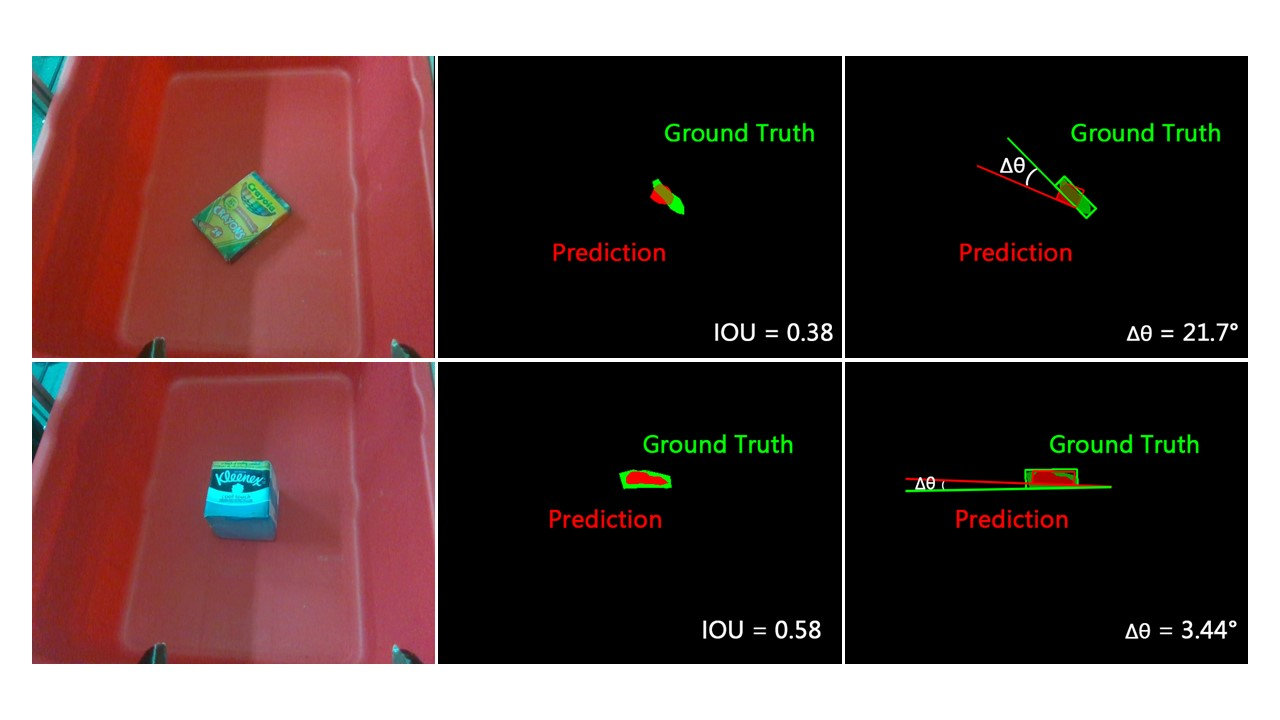
\includegraphics[height=!, width=1.0\linewidth, keepaspectratio=true]
	{./figures/iou_deltatheta.jpg}
  \caption{品牌文字語意切割的IoU與$\Delta\theta$範例。低IoU與會造成較大的$\Delta\theta$,並可能直接影響夾取可行性系統,造成之後的主動式操作系統夾取失敗。反之亦然,IoU愈高,則$\Delta\theta$愈小,夾取可行性預測將愈準確。}
  \label{figure:iou_deltatheta}
\end{figure}

本研究設計了表格~\ref{tbl:segmentation},縱軸為資料庫的所有子測試集,用來測試品牌文字切割模型,並以雜亂、遮蔽情況為標準,由簡單到複雜往下排列,橫軸則為評量的標準,第一部分為以場景(圖片)為單位的評估。這部分以F-score評估模型對整體圖片品牌文字切割的準確度。而第二部分則以所有場景中的所有品牌文字為單位,如此設計的原因是夾取可行性評估是以單一品牌文字預測標注遮罩與姿態作為線索,因此本研究十分重視對於每一個品牌文字語意切割預測的表現結果。在表格中有提供每一個子資料集所出現的可視的品牌文字數量、以及每個品牌文字預期結果與人為標注結果(groundtruth)的比較,並以IoU進行評量。依照人感官而言,IoU大於50\%,已經是很好的結果,看起來十分接近,因此本實驗預期整理出IoU大於50\%比例,並基於品牌文字皆為單行,可用旋轉矩形框住比擬的假設,針對這些品牌文字切割遮罩以一個旋轉矩形框住,去分析預測結果與真實標注的$\Delta\theta$(~\ref{figure:iou_deltatheta})。

\begin{table}[tb]
\centering
\caption{品牌文字語意切割模型評估表. Scene: 場景的數量, Vis. BN: 可是品牌文字的數量, Num.: 品牌文字IoU 小於 0.5的數量。}
\label{tbl:segmentation}
\tabcolsep=4pt
\begin{tabular}{l|cc|crcc}
\hline
                               & \multicolumn{2}{c|}{Image-level}                         & \multicolumn{4}{c}{Brandname-level}                                                                                        \\ \hline
\multirow{2}{*}{Benchmark}     & \multirow{2}{*}{Scene}    & \multirow{2}{*}{F-score}     & \multirow{2}{*}{Vis. BN}     & \multicolumn{1}{|c|}{IoU $<$ 0.5} & \multicolumn{2}{c}{IoU $\ge$ 0.5}                                  \\ \cline{5-7}
                               &                           &                              &                         & \multicolumn{1}{|c|}{Num. (\%)}        & \multicolumn{1}{c|}{Ave. IoU} & \multicolumn{1}{c}{$\Delta$$\theta$} \\ \hline
Single-1                       & 50                        & 0.70                & 50                      & 7  (14\%)                         & 0.72                          &  5.45                               \\
Duplicated-2                   & 90                        & 0.66                         & 145                     & 32 (22\%)                         & 0.71                          &  5.91                               \\
Multiple-2                     & 90                        & 0.66                         & 159                     & 36 (23\%)                         & 0.70                          &  5.64                               \\
Clutter-3                      & 20                        & 0.62                         & 31                      & 7  (23\%)                         & 0.73                          &  7.14                               \\
Clutter-5                      & 20                        & 0.60                         & 32                      & 11 (34\%)                         & 0.66                          &  7.77                               \\
Clutter-7                      & 20                        & 0.53                         & 59                      & 17 (29\%)                         & 0.70                          &  7.90                               \\ \hline
\end{tabular}
\end{table}

\subsection{實驗結果與討論}
整體上來說,此實驗證明了透過有限定範圍角度的品牌文字標注方法,可以訓練出具旋轉差異性的品牌文字切割模型,雖然仍有誤判情況發生,但是已可應用於主動式操作系統。此外,雖然在~\cite{zeng2016multi}的文獻中提出用單一物品於單一場景的訓練資料進行訓練,能在多物品複雜的場景中有好的成效,但參考表格中F-score一欄,可發現物體愈多,愈嚴重的雜亂情況下,會造成逐漸降低的F-score。同樣的以品牌文字為單位的評估中,雜亂環境也會增加預測出低IOU($ \le$ 0.5)的比率,以及惡化預測出高IOU($ \ge$  0.5)的品牌文字$\Delta\Theta$的大小,這些都會影響之後的主動式操作系統。

\subsection{失敗案例分析}
本研究觀察單一品牌文字偵測IoU$ \le$ 0.5之失敗案例,共將常出現之失敗案例分為四類。第一類(a)為不完整的遮罩。不完整的遮罩容易會造成之後,無論位置或是文字方向,品牌姿態預測的誤差。第二類(b)為類別的誤判,在此部分,不僅雖然品牌文字的部分有被偵測,但卻預測錯類別,會導致之後夾取與放置的方式錯誤,造成夾取失敗或是放錯格子的問題。第3類(c)為角度的誤判。一張圖片會以4個不同旋轉角度旋轉後再預測,最後整合為同一張圖片。此類的誤判是在錯誤的角度誤判到品牌文字,雖然偵測到品牌文字,也有正確的類別,卻會造成品牌文字方向的預測失敗。第4類(d)在商品的其餘部分偵測出品牌文字。這一類情況容易發生於較為雜亂的環境中。





\begin{figure}[ht]
	\centering
	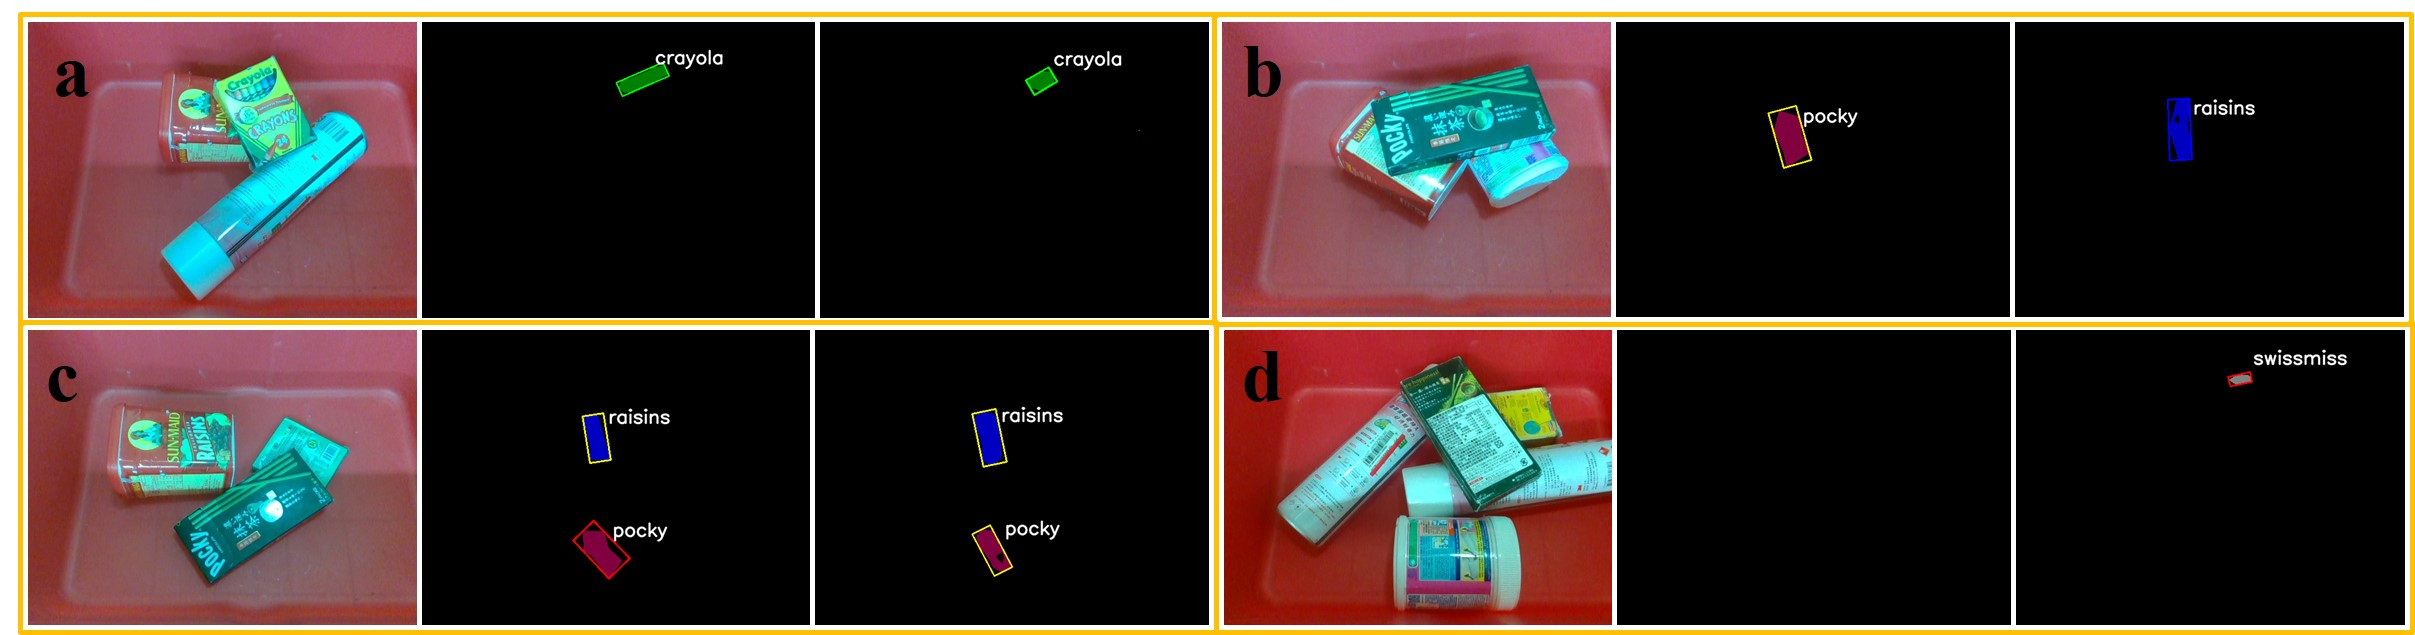
\includegraphics[height=!, width=1.0\linewidth, keepaspectratio=true]
	{./figures/failure_case.jpg}
  \caption{語意切割模型失敗範例。以品牌文字為單元,並以IoU = 0.5為門檻,定義小於0.5者為失敗的語意切割。本圖中共介紹4類常出現的失敗案例。}
  \label{figure:failure_case}
\end{figure}

\section{主動式操作系統評估}
本研究的第2個貢獻是開發主動式操作系統,此系統可開發目的為希望處理物體被遮蔽的情況,並有效達到特定姿態夾取與放置的任務,意思是透過第一次的夾取,能提升最後商品以特地姿態夾取放置的成功率。因此在本次實驗中採用測試集場景作為實驗場域,與baseline方法進行比較。本實驗預期能有系統的評估主動式操作系統的效果,並找出問題,作為未來改善空間。此實驗希望能有效回答1.主動式操作系統能否解決物品與品牌文字被遮蔽的問題。2.經由第一次夾取至空曠空間後,第二次的夾取放置成功率能否比擬baseline演算法。


\subsection{實驗設計}
本研究實驗主要目的為評估主動式操作系統成功率,共有6個測試場域集。實驗架設方式乃參考測試集場景,將物體放置成相同的位置擺法,接著藉由主動式操作系統或是baseline方法執行特定上架任務。物品必須被放置規定格子,並品牌文字朝前,才算成功。本研究設計了表格~\ref{table:active_manipulation_evaluation},去比較主動式操作系統與baseline的成功率。表格縱軸為場景測試集,後3個子測試集再細分為品牌文字朝上的與品牌文字朝下的,去分析品牌文字朝上或朝下對於主動式操作系統的影響程度。在橫軸部分,為baseline與主動式操作系統的每一個動作。希望透過這個表格去解析系統的特性。表格中夾取成功(Pick Success),定義為物品有被成功夾取,並直到放置前沒有掉落。而放置成功(Place Success),定義為物品被放置於指定的格子中,並且品牌文字朝外。

\begin{table}[bt]
\centering
\caption{定姿態夾取與放置演算法比較。誠如商品語意資料集段落所述,所有品牌文字於子測試集中場景Single-1、Duplicated-2、Multiple-3皆朝上(BN-UP)。而在其餘3個子測試集中,品牌文字有些朝上或有些朝下(BN-DOWN)。本研究發現Baseline方法在不雜亂場景(Single-1、Duplicated-2、Multiple-3)有很好的成效,但在雜亂環境中成效卻非常差,尤其是針對品牌文字朝下的物品。主動式操作系統則證明了能有效處理雜亂環境:能將物品從雜亂環境中夾出,在做特定姿態夾取動作。}
\begin{tabular}{ll|ll|lll}
\hline
\multicolumn{2}{l}{} & \multicolumn{2}{c}{Baseline} & \multicolumn{3}{c}{Active} \\
\hline
\textbf{} & Trials & \begin{tabular}[c]{@{}l@{}}Pick\\ Succ.\end{tabular} & \begin{tabular}[c]{@{}l@{}}Place\\ Succ.\end{tabular} & \begin{tabular}[c]{@{}l@{}}First \\ Pick \\ Succ.\end{tabular} & \begin{tabular}[c]{@{}l@{}}Second \\ Pick \\ Succ.\end{tabular} & \begin{tabular}[c]{@{}l@{}}Place\\ Succ.\end{tabular} \\
\hline
%\textbf{ALL-BN-UP} & 410       &               &               &         & & \\
\textbf{Single-1}        & 50        & \textbf{0.92} & \textbf{0.88} & - & -& -\\
\hline
\textbf{Duplicated-2}    & 180       & 0.82          & 0.76 & - & - & - \\
\hline
\textbf{Multiple-2}      & 180       & 0.81          & 0.69 & - & - & -\\
\hline
\textbf{Clutter-3} & 60 & & & & & \\
BN-UP & 33 & 0.48 & \textbf{0.39} & 0.88 & 0.82 & \textbf{0.73} \\
BN-DOWN & 27 & - & - & 0.85 & 0.59 & 0.59 \\
\hline
\textbf{Clutter-5} & 100 & & & & & \\
BN-UP & 35 & 0.31 & \textbf{0.26} & 0.80 & 0.57 & \textbf{0.49} \\
BN-DOWN & 65 & - & - & 0.75 & 0.45 & 0.37 \\
\hline
\textbf{Clutter-7} & 140 & & & & & \\
BN-UP & 74 & 0.23 & \textbf{0.19} & 0.74 & 0.49 & \textbf{0.43} \\
BN-DOWN & 66 & - & - & 0.74 & 0.38 & 0.33 \\
\hline
\end{tabular}
\label{table:active_manipulation_evaluation}
\end{table}


\subsection{實驗結果與討論}

\paragraph{Baseline 可有效處理單一物體的場景。於雜亂(多物體)環境則不然}
藉由實驗,於Single-1場景中,可了解baseline方法,對於單物體,且無遮蔽的環境,無論是夾取行為,都有很高的成功率(夾取達到0.92而放置達到0.88),但當環境複雜度提高(物體增加為2個時),於duplicated-2、Multiple-2場景中,放置成功率直接分別下降0.12與0.19。因此可發現Baseline對於雜亂環境相當敏感。

\paragraph{主動式操作系統對於雜亂環境的穩健性評估}
觀察主動式操作系統於測試場景Clutter-3的表現,無論是針對品牌文字朝上或朝下的物品,第一次夾取成功率都高達0.85以上。在愈複雜的環境(Clutter-5、Clutter-7)仍有0.74以上,可以證明主動式操作系統,藉由雙手臂協作方式,可以有效處理複雜的環境還有品牌文字朝下的狀況。此外藉由Baseline在Clutter-3、Clutter-5、Clutter-7場景低於0.5的成功率,也足以證明即使品牌文字朝上,要在雜亂環境中進行特定姿態的夾取行為,仍是十分困難,因此需要雙手臂的協作方式。在放置的成功率的比較中,主動式操作任務在品牌文字可視的情況下,比起baseline,在Clutter-3、Clutter-5、 Clutter-7也分別超出34\%、23\%、24\%。

\subsection{失敗案例分析}
主動式操作系統是2階段夾取放置行為,而第一次的夾取與放置行為對於第2次的夾取任務十分重要。換句話說,若第一次夾取或放置方式失敗,導致第2次無法成功觀察品牌文字,或是無法找到有效的夾取點,便會造成任務失敗。本部分將分析第一次使用吸盤夾爪夾取物品常出現之3個失敗案例:
\begin{itemize}
\item 第一個案例為吸盤夾爪系統基於品牌文字為線索進行夾取可行性預測結果,但由於品牌文字面積範圍較小,且該場景品牌文字在圓柱體上。圓柱體比起長方體,原本便較少夾取點可進行夾取,適合的夾取點只有圓柱體曲面法向量垂直吸盤夾取方向向量的小範圍面積。
\item 第二個範例為在品牌文字不可視的情況下,糟糕的物品語意切割結果會影響夾取可行性預測。導致預測出不好的夾取點,不好的夾取點會造成無法夾取物品,或夾取物品後移動時容易掉落。此外在不穩定的首次夾取,可能在第2次夾取時,物品鬆脫造成夾取姿態錯誤,最後放置失敗。
\item 第三個範例則是在品牌文字不可視時,相同物品也相鄰的場景中。語意切割模型準確偵測分類物品,單由於相鄰的商品皆被分為同一類,無法切割成不同物體。因此在點雲分析時,兩個物體點雲同時被納入分析,最後得出相鄰的區域作為夾取點
,導致夾取失敗。
\end{itemize}



\begin{figure}
  \centering
  \begin{subfigure}[b]{0.8\textwidth}
    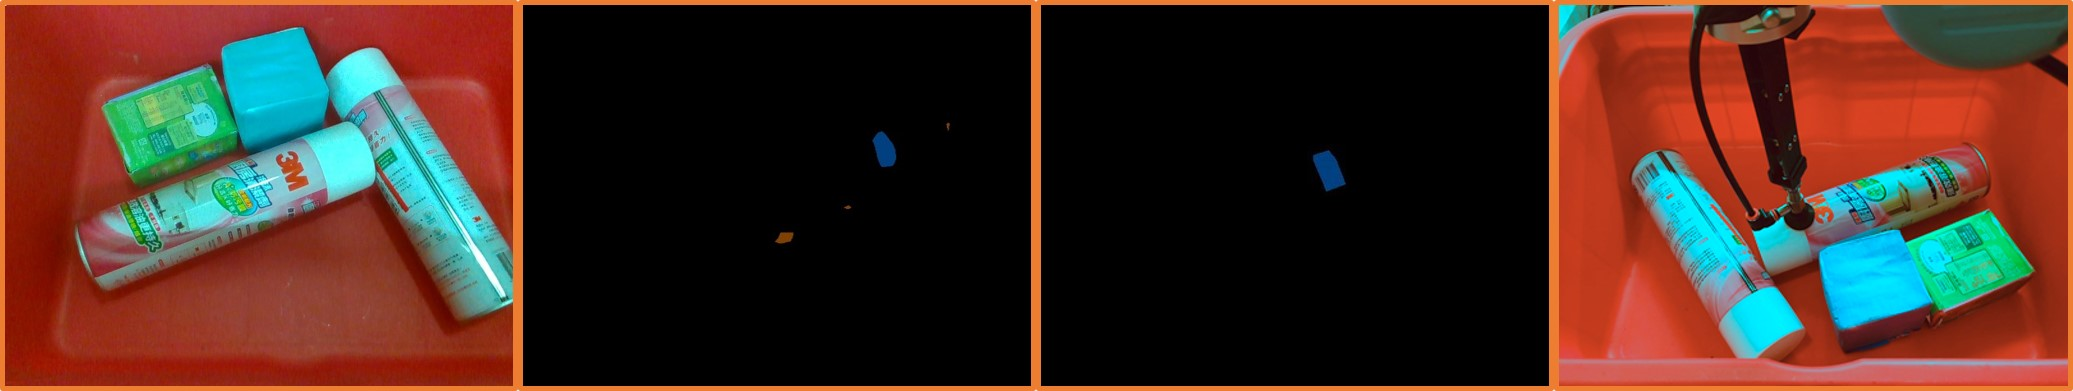
\includegraphics[width=\textwidth]{./figures/5_obj_8_suction_fail_2.jpg}
    \caption{Brandname is small and close to edge.}
    \label{fig:cylinder_suction_fail}
  \end{subfigure}
  \begin{subfigure}[b]{0.8\textwidth}
    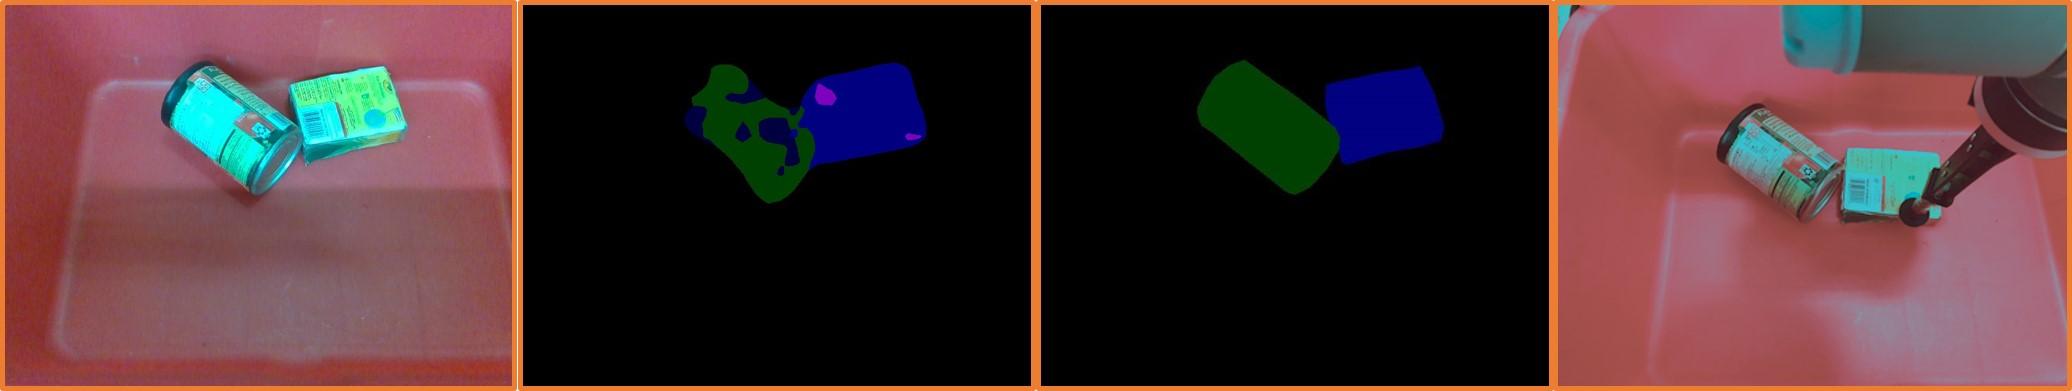
\includegraphics[width=\textwidth]{./figures/5_obj_13_suction_fail_3.jpg}
    \caption{Object segmentation (low precision or high false positives).}
    \label{fig:cuboid_suction_fail}
  \end{subfigure}
  \begin{subfigure}[b]{0.8\textwidth}
    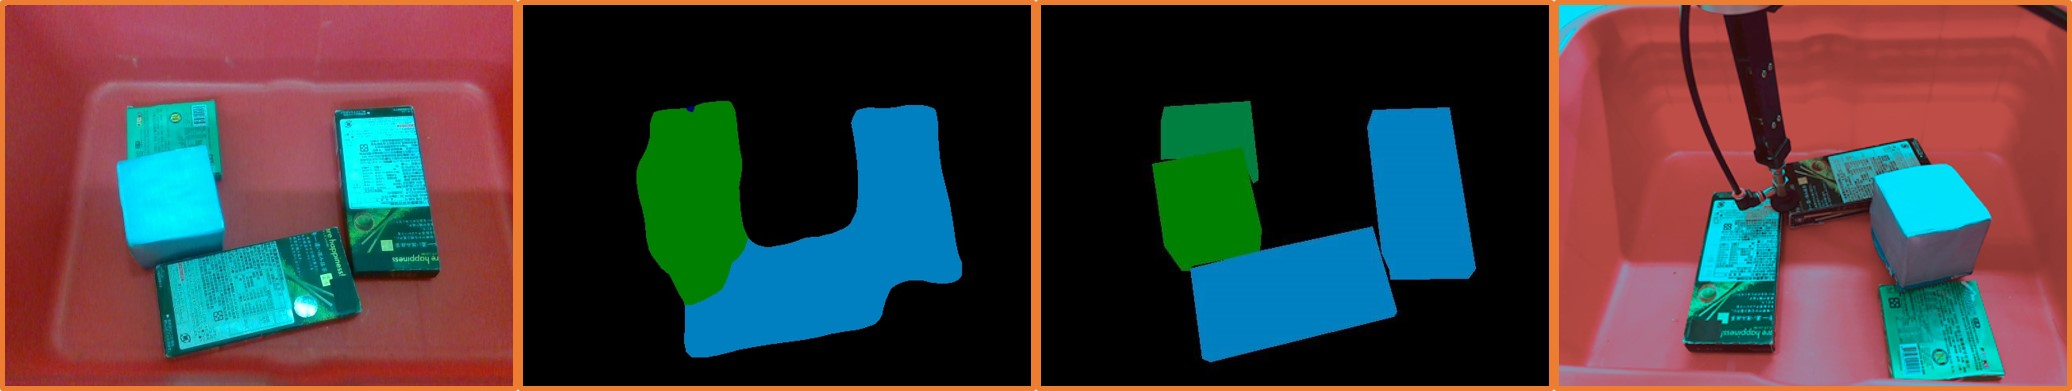
\includegraphics[width=\textwidth]{./figures/5_obj_14_suction_fail_1.jpg}
    \caption{Duplicated objects while brandname facing downward.}
    \label{fig:adjacent_suction_fail}
  \end{subfigure}
  \caption{吸盤夾爪吸取物品的常見失敗案例。共舉例3種不同常見例子,每個例子從左而右分別是輸入圖片、品牌文字或物品遮罩、Groundtruth標注、以及吸盤夾爪的行為。
}
  \label{fig:failure}
\end{figure}
